\chapter{Аналитическая часть}

\section{Анализ предметной области}

Поиск мероприятий для совместного досуга связан с выбором тематики, места и времени проведения. Объявления размещаются в разных группах и общих лентах, поэтому пользователю приходится просматривать множество публикаций, чтобы найти подходящее мероприятие. Если дата, адрес и условия участия указаны неполно или в разных сообщениях, сравнение вариантов занимает дополнительное время.

Для организации мероприятия нужно указать его тему, время и место проведения, опубликовать описание и учитывать участников. В общей ленте объявление быстро теряется среди других записей, а изменение сведений и учет откликов затруднены. Для упрощения этих задач необходима система, в которой можно быстро найти мероприятия по интересам, городу и дате, а также разместить свое объявление и вести учет участников.

\section{Анализ известных решений}

Рассмотрим следующие существующие решения для поиска и организации мероприятий:
\begin{enumerate}[label=\arabic*)]
    \item Meetup -- сервис публикации и поиска встреч по интересам с учетом участников~\cite{meetup-create,meetup-search,meetup-account,meetup-chat};
    \item Mobilizon -- приложение для создания мероприятий, поиска и управления участием; организатор может разрешить запись без учетной записи~\cite{mobilizon-create,mobilizon-search,mobilizon-about,mobilizon-share};
    \item Timepad -- сервис публикации и поиска мероприятий, регистрации участников и продажи билетов~\cite{timepad-create,timepad-search,timepad-product};
    \item группы в социальных сетях -- публикация объявлений в ленте группы с обсуждением в комментариях.
\end{enumerate}

Критерии сравнения и результаты представлены в таблицах~\ref{tab:criteria} и~\ref{tab:analogues}. Для групп рассматриваются обычные публикации в популярных социальных сетях, без отдельных сервисов мероприятий. Универсальность означает возможность размещения мероприятий разных тематик.

\begin{table}[H]
    \caption{Критерии сравнения известных решений}
    \label{tab:criteria}
    \begin{tabularx}{\textwidth}{|p{4.8cm}|X|}
        \hline
        \textbf{Критерий} & \textbf{Описание} \\
        \hline
        Доступность в РФ & Возможность пользоваться приложением из России \\
        \hline
        Интеграция \mbox{с соцсетями} & Средства публикации, регистрации или общения через соцсети и мессенджеры \\
        \hline
        Универсальность & Размещение мероприятий разных тематик \\
        \hline
        Запись без аккаунта & Подтверждение участия без предварительного создания учетной записи \\
        \hline
        Фильтры поиска & Поиск мероприятий по месту, тематике и времени проведения \\
        \hline
    \end{tabularx}
\end{table}

\begin{table}[H]
    \caption{Результаты сравнения известных решений}
    \label{tab:analogues}
    \small
    \setlength{\tabcolsep}{4pt}
    \begin{tabularx}{\textwidth}{|p{3.8cm}|Y|Y|Y|Y|Y|}
        \hline
        \textbf{Критерий} & \textbf{Meetup} & \textbf{Mobilizon} & \textbf{Timepad} & \textbf{\shortstack{Группы\\соцсетей}} & \textbf{JoinUp} \\
        \hline
        Доступность в РФ & Нет & Нет & Да & Да & Да \\
        \hline
        Интеграция \mbox{с соцсетями} & Нет & Нет & Да & Да & Да \\
        \hline
        Универсальность & Да & Да & Да & Нет & Да \\
        \hline
        Запись без аккаунта & Нет & Да & Да & Нет & Нет \\
        \hline
        Фильтры поиска & Нет & Да & Да & Нет & Да \\
        \hline
    \end{tabularx}
\end{table}

\section{Формализация данных}

Основные группы данных представлены в таблице~\ref{tab:entities}. Каждая запись имеет идентификатор. Участие пользователей и принадлежность мероприятий к категориям образуют связи <<многие ко многим>>.

\begin{table}[H]
    \caption{Группы данных и сведения о них}
    \label{tab:entities}
    \begin{tabularx}{\textwidth}{|p{3.7cm}|X|}
        \hline
        \textbf{Данные} & \textbf{Сведения} \\
        \hline
        Пользователь & Имя, возраст, логин, хеш пароля, город, Telegram, роль, аватар, дата регистрации \\
        \hline
        Мероприятие & Название, описание, город, время, организатор, локация, чат, обложка, признак удаления \\
        \hline
        Участие & Пользователь, мероприятие, роль участника \\
        \hline
        Локация & Название, адрес, координаты \\
        \hline
        Категория & Название, вышестоящая категория \\
        \hline
        Изображение & Имя файла, содержимое \\
        \hline
        Отзыв & Автор, мероприятие, оценка, текст, дата \\
        \hline
        Журнал удаления & Мероприятие, время удаления \\
        \hline
    \end{tabularx}
\end{table}

На рисунке~\ref{fig:chen} представлена исходная диаграмма предметной области. Реализованная БД дополнена отзывами и журналом удаления; показанные на схеме подписка и дата вступления не используются приложением.

\begin{figure}[H]
    \centering
    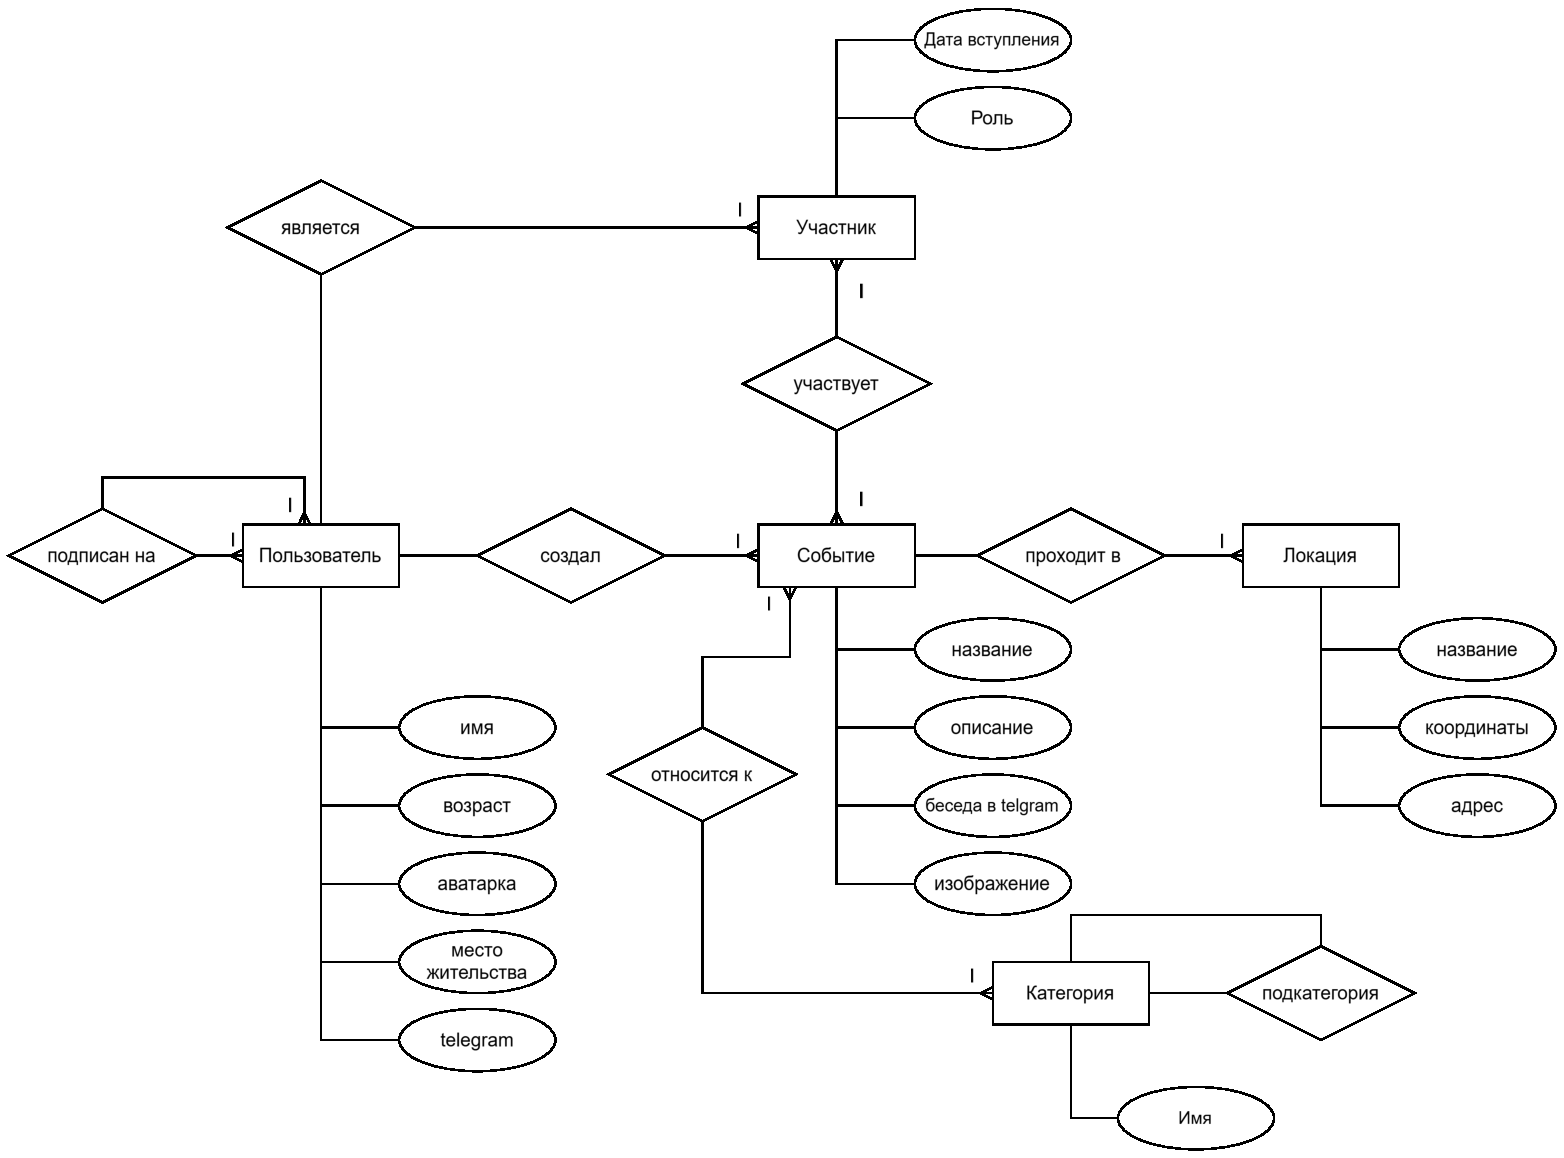
\includegraphics[width=\textwidth]{../images/ER.pdf}
    \caption{Диаграмма сущность-связь}
    \label{fig:chen}
\end{figure}

\section{Формализация ролей}

Роли приложения приведены в таблице~\ref{tab:roles}, их действия -- на рисунке~\ref{fig:use-cases}.

\begin{table}[H]
    \caption{Роли пользователей приложения}
    \label{tab:roles}
    \begin{tabularx}{\textwidth}{|p{3.5cm}|X|}
        \hline
        \textbf{Роль} & \textbf{Возможности} \\
        \hline
        Гость & Регистрация, вход, просмотр объявлений и отзывов \\
        \hline
        Пользователь & Поиск, создание и изменение своих мероприятий, участие, отзывы, работа с профилем \\
        \hline
        Администратор & Действия пользователя, изменение и удаление чужих мероприятий \\
        \hline
    \end{tabularx}
\end{table}

Роли БД задают права чтения, изменения и администрирования данных. Сервер подключается с пользовательской ролью БД; права на объявления проверяет приложение.

\begin{figure}[p]
    \centering
    \singlespacing
    \begin{tikzpicture}[
        font=\small\linespread{1}\selectfont,
        usecase/.style={draw, ellipse, text width=5.4cm, minimum height=1cm, inner ysep=0pt, align=center},
        actorlabel/.style={align=center, text width=3.3cm},
        every path/.style={line width=0.5pt}
    ]
        \draw (3,-0.9) rectangle (14,18.5);
        \node at (8.5,18) {Приложение JoinUp};
        \node[usecase] (register) at (8.7,17) {Зарегистрироваться};
        \node[usecase] (login) at (8.7,15.3) {Войти в приложение};
        \node[usecase] (search) at (8.7,13.6) {Найти и просмотреть\\мероприятие};
        \node[usecase] (create) at (8.7,11.9) {Создать мероприятие};
        \node[usecase] (edit) at (8.7,10.2) {Изменить или удалить\\свое мероприятие};
        \node[usecase] (join) at (8.7,8.5) {Присоединиться или отказаться от участия};
        \node[usecase] (lists) at (8.7,6.8) {Просмотреть свои мероприятия};
        \node[usecase] (reviews) at (8.7,5.1) {Просмотреть или оставить отзыв};
        \node[usecase] (profile) at (8.7,3.4) {Просмотреть профиль и изменить свои данные};
        \node[usecase] (moderate) at (8.7,0.5) {Изменить или удалить чужое мероприятие};

        \foreach \name/\y/\caption in {guest/16/Гость, user/8.5/Пользователь, admin/0.5/Администратор} {
            \coordinate (\name) at (1,\y);
            \draw (1,\y+0.6) circle (0.18);
            \draw (1,\y+0.42) -- (1,\y-0.2);
            \draw (0.6,\y+0.2) -- (1.4,\y+0.2);
            \draw (0.65,\y-0.65) -- (1,\y-0.2) -- (1.35,\y-0.65);
            \node[actorlabel] at (1,\y-0.95) {\caption};
        }
        \draw (guest) -- (register.west);
        \draw (guest) -- (login.west);
        \foreach \target in {search,create,edit,join,lists,reviews,profile}
            \draw (user) -- (2.8,8.5) -- (\target.west);
        \draw (admin) -- (moderate.west);
        \draw[-{Triangle[open, length=4mm, width=3mm]}] (1,1.3) -- (1,7.2);
    \end{tikzpicture}
    \caption{Диаграмма прецедентов}
    \label{fig:use-cases}
\end{figure}
\clearpage

\section{Анализ моделей баз данных}

Иерархическая модель представляет данные деревом: у подчиненной записи один родитель~\cite{data-modeling}. Она подходит для категорий, но связи пользователей с несколькими мероприятиями требуют дополнительных ссылок либо дублирования данных.

Документная модель хранит объекты с вложенными данными или ссылками~\cite{document-model}. Мероприятие можно хранить вместе с участниками, однако при копировании сведений о пользователе их изменение потребует обновления нескольких документов.

Реляционная модель представляет данные таблицами, связанными ключами~\cite{data-modeling}. Для JoinUp выбирается эта модель: состав атрибутов определен, участие и категории задаются отдельными отношениями, поиск выполняется отбором и соединением записей, рейтинг -- агрегированием оценок.

\section{Формализация задачи}

Необходимо разработать реляционную БД и приложение для публикации и поиска мероприятий, учета участия и отзывов. Требуется обеспечить целостность данных, разграничение прав и запись фактов удаления объявлений триггером. После реализации необходимо проверить основные операции и исследовать зависимость среднего времени поиска от количества мероприятий с индексом по основным фильтрам и без него.
